\documentclass[twoside]{book}

% Packages required by doxygen
\usepackage{fixltx2e}
\usepackage{calc}
\usepackage{doxygen}
\usepackage[export]{adjustbox} % also loads graphicx
\usepackage{graphicx}
\usepackage[utf8]{inputenc}
\usepackage{makeidx}
\usepackage{multicol}
\usepackage{multirow}
\PassOptionsToPackage{warn}{textcomp}
\usepackage{textcomp}
\usepackage[nointegrals]{wasysym}
\usepackage[table]{xcolor}

% NLS support packages
\usepackage[spanish]{babel}
% Font selection
\usepackage[T1]{fontenc}
\usepackage[scaled=.90]{helvet}
\usepackage{courier}
\usepackage{amssymb}
\usepackage{sectsty}
\renewcommand{\familydefault}{\sfdefault}
\allsectionsfont{%
  \fontseries{bc}\selectfont%
  \color{darkgray}%
}
\renewcommand{\DoxyLabelFont}{%
  \fontseries{bc}\selectfont%
  \color{darkgray}%
}
\newcommand{\+}{\discretionary{\mbox{\scriptsize$\hookleftarrow$}}{}{}}

% Page & text layout
\usepackage{geometry}
\geometry{%
  a4paper,%
  top=2.5cm,%
  bottom=2.5cm,%
  left=2.5cm,%
  right=2.5cm%
}
\tolerance=750
\hfuzz=15pt
\hbadness=750
\setlength{\emergencystretch}{15pt}
\setlength{\parindent}{0cm}
\setlength{\parskip}{3ex plus 2ex minus 2ex}
\makeatletter
\renewcommand{\paragraph}{%
  \@startsection{paragraph}{4}{0ex}{-1.0ex}{1.0ex}{%
    \normalfont\normalsize\bfseries\SS@parafont%
  }%
}
\renewcommand{\subparagraph}{%
  \@startsection{subparagraph}{5}{0ex}{-1.0ex}{1.0ex}{%
    \normalfont\normalsize\bfseries\SS@subparafont%
  }%
}
\makeatother

% Headers & footers
\usepackage{fancyhdr}
\pagestyle{fancyplain}
\fancyhead[LE]{\fancyplain{}{\bfseries\thepage}}
\fancyhead[CE]{\fancyplain{}{}}
\fancyhead[RE]{\fancyplain{}{\bfseries\leftmark}}
\fancyhead[LO]{\fancyplain{}{\bfseries\rightmark}}
\fancyhead[CO]{\fancyplain{}{}}
\fancyhead[RO]{\fancyplain{}{\bfseries\thepage}}
\fancyfoot[LE]{\fancyplain{}{}}
\fancyfoot[CE]{\fancyplain{}{}}
\fancyfoot[RE]{\fancyplain{}{\bfseries\scriptsize Generado por Doxygen }}
\fancyfoot[LO]{\fancyplain{}{\bfseries\scriptsize Generado por Doxygen }}
\fancyfoot[CO]{\fancyplain{}{}}
\fancyfoot[RO]{\fancyplain{}{}}
\renewcommand{\footrulewidth}{0.4pt}
\renewcommand{\chaptermark}[1]{%
  \markboth{#1}{}%
}
\renewcommand{\sectionmark}[1]{%
  \markright{\thesection\ #1}%
}

% Indices & bibliography
\usepackage{natbib}
\usepackage[titles]{tocloft}
\setcounter{tocdepth}{3}
\setcounter{secnumdepth}{5}
\makeindex

% Hyperlinks (required, but should be loaded last)
\usepackage{ifpdf}
\ifpdf
  \usepackage[pdftex,pagebackref=true]{hyperref}
\else
  \usepackage[ps2pdf,pagebackref=true]{hyperref}
\fi
\hypersetup{%
  colorlinks=true,%
  linkcolor=blue,%
  citecolor=blue,%
  unicode%
}

% Custom commands
\newcommand{\clearemptydoublepage}{%
  \newpage{\pagestyle{empty}\cleardoublepage}%
}

\usepackage{caption}
\captionsetup{labelsep=space,justification=centering,font={bf},singlelinecheck=off,skip=4pt,position=top}

%===== C O N T E N T S =====

\begin{document}

% Titlepage & ToC
\hypersetup{pageanchor=false,
             bookmarksnumbered=true,
             pdfencoding=unicode
            }
\pagenumbering{roman}
\begin{titlepage}
\vspace*{7cm}
\begin{center}%
{\Large Laboratorio de P\+R\+O2. Caso de estudio\+: experimentos inmunologicos. \\[1ex]\large v7.\+0 13-\/11-\/2017 }\\
\vspace*{1cm}
{\large Generado por Doxygen 1.8.11}\\
\end{center}
\end{titlepage}
\clearemptydoublepage
\tableofcontents
\clearemptydoublepage
\pagenumbering{arabic}
\hypersetup{pageanchor=true}

%--- Begin generated contents ---
\chapter{Página principal}
\label{index}\hypertarget{index}{}En este ejemplo se construye un programa modular que ofrece un menú de opciones para gestionar una lavadora. Se introducen las clases {\itshape \mbox{\hyperlink{class_lavadora}{Lavadora}}}, {\itshape \mbox{\hyperlink{class_cubeta}{Cubeta}}} y {\itshape \mbox{\hyperlink{class_prenda}{Prenda}}}.

Sólo se documentan elementos públicos. En una próxima sesión se verá un ejemplo de proyecto completamente documentado, incluyendo los elementos privados. 
\chapter{Índice de clases}
\doxysection{Lista de clases}
Lista de las clases, estructuras, uniones e interfaces con una breve descripción\+:\begin{DoxyCompactList}
\item\contentsline{section}{\mbox{\hyperlink{class_alfabeto}{Alfabeto}} }{\pageref{class_alfabeto}}{}
\item\contentsline{section}{\mbox{\hyperlink{class_c_alfabetos}{C\+Alfabetos}} }{\pageref{class_c_alfabetos}}{}
\item\contentsline{section}{\mbox{\hyperlink{class_c_mensajes}{C\+Mensajes}} }{\pageref{class_c_mensajes}}{}
\item\contentsline{section}{\mbox{\hyperlink{class_mensaje}{Mensaje}} }{\pageref{class_mensaje}}{}
\end{DoxyCompactList}

\chapter{Indice de archivos}
\doxysection{Llista dels Fitxers}
Aquesta és la llista de tots els fitxers acompanyats amb breus descripcions\+:\begin{DoxyCompactList}
\item\contentsline{section}{\mbox{\hyperlink{_alfabeto_8hh}{Alfabeto.\+hh}} \\*Especificación de la clase alfabeto }{\pageref{_alfabeto_8hh}}{}
\item\contentsline{section}{\mbox{\hyperlink{_bin_tree_8hh}{Bin\+Tree.\+hh}} }{\pageref{_bin_tree_8hh}}{}
\item\contentsline{section}{\mbox{\hyperlink{_c_alfabetos_8hh}{C\+Alfabetos.\+hh}} \\*Especificación de la clase conjunto de alfabetos }{\pageref{_c_alfabetos_8hh}}{}
\item\contentsline{section}{\mbox{\hyperlink{_c_mensajes_8hh}{C\+Mensajes.\+hh}} \\*Especificación de la clase conjunto de mensajes }{\pageref{_c_mensajes_8hh}}{}
\item\contentsline{section}{\mbox{\hyperlink{_mensaje_8hh}{Mensaje.\+hh}} \\*Especificación de la clase mensaje }{\pageref{_mensaje_8hh}}{}
\item\contentsline{section}{\mbox{\hyperlink{_program_8cc}{Program.\+cc}} \\*Programa main }{\pageref{_program_8cc}}{}
\end{DoxyCompactList}

\chapter{Documentación de las clases}
\hypertarget{class_celula}{}\section{Referencia de la Clase Celula}
\label{class_celula}\index{Celula@{Celula}}


Representa el conjunto de características y operaciones de las células.  


\subsection*{Métodos públicos}
\begin{DoxyCompactItemize}
\item 
\hyperlink{class_celula_a3c5017fbcec8cb564acc666aa7e21206}{Celula} ()
\begin{DoxyCompactList}\small\item\em Creadora por defecto. \end{DoxyCompactList}\item 
int \hyperlink{class_celula_a3dd8be98f1548b02696e2fc32b8d19b4}{lucha\+\_\+celulas} (const \hyperlink{class_celula}{Celula} \&c2) const 
\begin{DoxyCompactList}\small\item\em Consultora que determina el resultado de la lucha entre dos células. \end{DoxyCompactList}\item 
bool \hyperlink{class_celula_a4e97c60a207191b2cc951ccdf245df4b}{es\+\_\+vacia} () const 
\begin{DoxyCompactList}\small\item\em Consultora que indica si la célula es vacía. \end{DoxyCompactList}\item 
int \hyperlink{class_celula_a872a679a68e462dabde1ea4fe5fbc0ad}{num\+\_\+param} ()
\begin{DoxyCompactList}\small\item\em Consultora del número de parámetros de una célula. \end{DoxyCompactList}\item 
void \hyperlink{class_celula_a5124ea0c0da24dfc295dcc428652ee43}{leer} (int N)
\begin{DoxyCompactList}\small\item\em Operación de lectura. \end{DoxyCompactList}\item 
void \hyperlink{class_celula_ae16a94d28e49affafd260405414f37ad}{escribir} () const 
\begin{DoxyCompactList}\small\item\em Operación de escritura. \end{DoxyCompactList}\end{DoxyCompactItemize}
\subsection*{Métodos públicos estáticos}
\begin{DoxyCompactItemize}
\item 
static int \hyperlink{class_celula_ad1f2960d79a418652964b6aeedaa8243}{id\+\_\+vacia} ()
\begin{DoxyCompactList}\small\item\em Consultora del identificador especial de células vacías. \end{DoxyCompactList}\end{DoxyCompactItemize}
\subsection*{Atributos privados}
\begin{DoxyCompactItemize}
\item 
int \hyperlink{class_celula_a0984a8b3deeed4979ed6f6141edc3c0c}{id}
\begin{DoxyCompactList}\small\item\em Identificador de la célula. \end{DoxyCompactList}\item 
int \hyperlink{class_celula_abda46be7b30a13909d9819c46238080b}{i\+\_\+tol}
\begin{DoxyCompactList}\small\item\em Indice de tolerancia. \end{DoxyCompactList}\item 
vector$<$ double $>$ \hyperlink{class_celula_a386c6da3af12b5662e3866675d60a4b7}{param}
\begin{DoxyCompactList}\small\item\em Parámetros de la célula. \end{DoxyCompactList}\end{DoxyCompactItemize}
\subsection*{Atributos privados estáticos}
\begin{DoxyCompactItemize}
\item 
static const int \hyperlink{class_celula_affff67b41ead0b1f3a3f4faad6c049ac}{I\+D\+\_\+\+V\+A\+C\+IA} = 0
\begin{DoxyCompactList}\small\item\em Identificador especial para células vacias. \end{DoxyCompactList}\end{DoxyCompactItemize}


\subsection{Descripción detallada}
Representa el conjunto de características y operaciones de las células. 

Ofrece la operación de lucha entre células y las operaciones de lectura y escritura.

Dado que vamos a necesitar leer árboles de células, definimos el concepto de célula vacía para disponer de un formato de entrada parecido al de las anteriores sesiones de laboratorio, en las que se emplea una \char`\"{}marca\char`\"{} para indicar la lectura de un árbol vacío. 

Definición en la línea 30 del archivo Celula.\+hh.



\subsection{Documentación del constructor y destructor}
\index{Celula@{Celula}!Celula@{Celula}}
\index{Celula@{Celula}!Celula@{Celula}}
\subsubsection[{\texorpdfstring{Celula()}{Celula()}}]{\setlength{\rightskip}{0pt plus 5cm}Celula\+::\+Celula (
\begin{DoxyParamCaption}
{}
\end{DoxyParamCaption}
)}\hypertarget{class_celula_a3c5017fbcec8cb564acc666aa7e21206}{}\label{class_celula_a3c5017fbcec8cb564acc666aa7e21206}


Creadora por defecto. 

\begin{DoxyPrecond}{Precondición}
cierto 
\end{DoxyPrecond}
\begin{DoxyPostcond}{Postcondición}
El resultado es una célula vacía, con índice de tolerancia cero y cero parámetros 
\end{DoxyPostcond}
\begin{DoxyParagraph}{Coste}
Constante 
\end{DoxyParagraph}


Definición en la línea 7 del archivo Celula.\+cc.


\begin{DoxyCode}
8 \{
9   \textcolor{comment}{// Inicializa una célula con el id de célula vacía}
10   \textcolor{keywordtype}{id} = \hyperlink{class_celula_affff67b41ead0b1f3a3f4faad6c049ac}{ID\_VACIA};
11   \hyperlink{class_celula_abda46be7b30a13909d9819c46238080b}{i\_tol} = 0;
12 \}
\end{DoxyCode}


\subsection{Documentación de las funciones miembro}
\index{Celula@{Celula}!lucha\+\_\+celulas@{lucha\+\_\+celulas}}
\index{lucha\+\_\+celulas@{lucha\+\_\+celulas}!Celula@{Celula}}
\subsubsection[{\texorpdfstring{lucha\+\_\+celulas(const Celula \&c2) const }{lucha_celulas(const Celula &c2) const }}]{\setlength{\rightskip}{0pt plus 5cm}int Celula\+::lucha\+\_\+celulas (
\begin{DoxyParamCaption}
\item[{const {\bf Celula} \&}]{c2}
\end{DoxyParamCaption}
) const}\hypertarget{class_celula_a3dd8be98f1548b02696e2fc32b8d19b4}{}\label{class_celula_a3dd8be98f1548b02696e2fc32b8d19b4}


Consultora que determina el resultado de la lucha entre dos células. 

\begin{DoxyPrecond}{Precondición}
El parámetro implícito (c1) y c2 tienen el mismo número de parámetros 
\end{DoxyPrecond}
\begin{DoxyPostcond}{Postcondición}
Retorna el resultado de la lucha entre c1 y c2, que vale 1 si y solo si c1 vence a c2; 2 si y solo si c2 vence a c1; 3 si y solo si no vence ninguna de las dos 
\end{DoxyPostcond}
\begin{DoxyParagraph}{Coste}
Lineal respecto al número de parámetros de una célula 
\end{DoxyParagraph}


Definición en la línea 14 del archivo Celula.\+cc.


\begin{DoxyCode}
15 \{
16 
17   \textcolor{keywordflow}{if} (\hyperlink{class_celula_a386c6da3af12b5662e3866675d60a4b7}{param}.size()!=c2.\hyperlink{class_celula_a386c6da3af12b5662e3866675d60a4b7}{param}.size()) \textcolor{keywordflow}{throw} PRO2Excepcio(\textcolor{stringliteral}{"Las dos células han de tener el mismo
       número de parámetros"});
18 
19   \textcolor{comment}{// Se trata de obtener la diferencia entre el número de posiciones de la primera}
20   \textcolor{comment}{// célula que superan a las de la segunda y viceversa. Después se compara dicha}
21   \textcolor{comment}{// diferencia con los indicadores de tolerancia.}
22   \textcolor{keywordtype}{int} i = 0; 
23   \textcolor{keywordtype}{int} dif = 0;
24 
25   \textcolor{comment}{// Inv: dif = diferencia entre el número de posiciones en [0..i-1] en que c1 supera a c2 }
26   \textcolor{comment}{// y viceversa, 0<=i<=param.size()}
27   
28   \textcolor{keywordflow}{while} (i < \hyperlink{class_celula_a386c6da3af12b5662e3866675d60a4b7}{param}.size()) \{
29     \textcolor{keywordflow}{if} (\hyperlink{class_celula_a386c6da3af12b5662e3866675d60a4b7}{param}[i] > c2.\hyperlink{class_celula_a386c6da3af12b5662e3866675d60a4b7}{param}[i]) ++dif;
30     \textcolor{keywordflow}{else} \textcolor{keywordflow}{if} (\hyperlink{class_celula_a386c6da3af12b5662e3866675d60a4b7}{param}[i] < c2.\hyperlink{class_celula_a386c6da3af12b5662e3866675d60a4b7}{param}[i]) --dif;
31     ++i;
32   \}
33   \textcolor{comment}{// Post1: dif = diferencia entre el número de posiciones totales en que }
34   \textcolor{comment}{// c1 supera a c2 y viceversa }
35   \textcolor{keywordtype}{int} n = 3;
36   \textcolor{keywordflow}{if} (dif > c2.\hyperlink{class_celula_abda46be7b30a13909d9819c46238080b}{i\_tol}) n = 1;
37   \textcolor{keywordflow}{else} \textcolor{keywordflow}{if} (dif < -\hyperlink{class_celula_abda46be7b30a13909d9819c46238080b}{i\_tol}) n = 2;
38   \textcolor{keywordflow}{return} n;
39 \}
\end{DoxyCode}
\index{Celula@{Celula}!es\+\_\+vacia@{es\+\_\+vacia}}
\index{es\+\_\+vacia@{es\+\_\+vacia}!Celula@{Celula}}
\subsubsection[{\texorpdfstring{es\+\_\+vacia() const }{es_vacia() const }}]{\setlength{\rightskip}{0pt plus 5cm}bool Celula\+::es\+\_\+vacia (
\begin{DoxyParamCaption}
{}
\end{DoxyParamCaption}
) const}\hypertarget{class_celula_a4e97c60a207191b2cc951ccdf245df4b}{}\label{class_celula_a4e97c60a207191b2cc951ccdf245df4b}


Consultora que indica si la célula es vacía. 

\begin{DoxyPrecond}{Precondición}
cierto 
\end{DoxyPrecond}
\begin{DoxyPostcond}{Postcondición}
El resultado indica si la célula es vacía o no 
\end{DoxyPostcond}
\begin{DoxyParagraph}{Coste}
Constante 
\end{DoxyParagraph}


Definición en la línea 41 del archivo Celula.\+cc.


\begin{DoxyCode}
42 \{
43   \textcolor{keywordflow}{return} \textcolor{keywordtype}{id} == \hyperlink{class_celula_affff67b41ead0b1f3a3f4faad6c049ac}{ID\_VACIA};
44 \}
\end{DoxyCode}
\index{Celula@{Celula}!num\+\_\+param@{num\+\_\+param}}
\index{num\+\_\+param@{num\+\_\+param}!Celula@{Celula}}
\subsubsection[{\texorpdfstring{num\+\_\+param()}{num_param()}}]{\setlength{\rightskip}{0pt plus 5cm}int Celula\+::num\+\_\+param (
\begin{DoxyParamCaption}
{}
\end{DoxyParamCaption}
)}\hypertarget{class_celula_a872a679a68e462dabde1ea4fe5fbc0ad}{}\label{class_celula_a872a679a68e462dabde1ea4fe5fbc0ad}


Consultora del número de parámetros de una célula. 

\begin{DoxyPrecond}{Precondición}
cierto 
\end{DoxyPrecond}
\begin{DoxyPostcond}{Postcondición}
El resultado es el número de parámetros de una célula 
\end{DoxyPostcond}
\begin{DoxyParagraph}{Coste}
Constante 
\end{DoxyParagraph}


Definición en la línea 46 del archivo Celula.\+cc.


\begin{DoxyCode}
46                      \{
47   \textcolor{keywordflow}{return} \hyperlink{class_celula_a386c6da3af12b5662e3866675d60a4b7}{param}.size();
48 \}
\end{DoxyCode}
\index{Celula@{Celula}!id\+\_\+vacia@{id\+\_\+vacia}}
\index{id\+\_\+vacia@{id\+\_\+vacia}!Celula@{Celula}}
\subsubsection[{\texorpdfstring{id\+\_\+vacia()}{id_vacia()}}]{\setlength{\rightskip}{0pt plus 5cm}int Celula\+::id\+\_\+vacia (
\begin{DoxyParamCaption}
{}
\end{DoxyParamCaption}
)\hspace{0.3cm}{\ttfamily [static]}}\hypertarget{class_celula_ad1f2960d79a418652964b6aeedaa8243}{}\label{class_celula_ad1f2960d79a418652964b6aeedaa8243}


Consultora del identificador especial de células vacías. 

\begin{DoxyPrecond}{Precondición}
cierto 
\end{DoxyPrecond}
\begin{DoxyPostcond}{Postcondición}
El resultado es el identificador de célula vacía 
\end{DoxyPostcond}
\begin{DoxyParagraph}{Coste}
Constante 
\end{DoxyParagraph}


Definición en la línea 50 del archivo Celula.\+cc.


\begin{DoxyCode}
51 \{
52   \textcolor{keywordflow}{return} \hyperlink{class_celula_affff67b41ead0b1f3a3f4faad6c049ac}{ID\_VACIA};
53 \}
\end{DoxyCode}
\index{Celula@{Celula}!leer@{leer}}
\index{leer@{leer}!Celula@{Celula}}
\subsubsection[{\texorpdfstring{leer(int N)}{leer(int N)}}]{\setlength{\rightskip}{0pt plus 5cm}void Celula\+::leer (
\begin{DoxyParamCaption}
\item[{int}]{N}
\end{DoxyParamCaption}
)}\hypertarget{class_celula_a5124ea0c0da24dfc295dcc428652ee43}{}\label{class_celula_a5124ea0c0da24dfc295dcc428652ee43}


Operación de lectura. 

\begin{DoxyPrecond}{Precondición}
N$>$0, el canal de entrada estándar contiene un entero; si dicho entero no corresponde a un identificador de célula vacía, a continuación contiene otro entero y N doubles 
\end{DoxyPrecond}
\begin{DoxyPostcond}{Postcondición}
El parámetro implícito pasa a tener un identificador (el primer entero del canal de entrada estándar); si éste no es el de una célula vacía, el p.\+i. también tendrá un índice de tolerancia y N parámetros nuevos, leídos del canal de entrada estándar 
\end{DoxyPostcond}
\begin{DoxyParagraph}{Coste}
Lineal respecto a N (número de parámetros de una célula) 
\end{DoxyParagraph}


Definición en la línea 55 del archivo Celula.\+cc.


\begin{DoxyCode}
56 \{
57   \textcolor{comment}{// Simplemente lee todos los componentes de la célula teniendo en cuenta que si }
58   \textcolor{comment}{// el identificador es cero se trata de una celula "marca" y no es necesario continuar leyendo.}
59 
60   \textcolor{keywordflow}{if} (N<=0) \textcolor{keywordflow}{throw} PRO2Excepcio(\textcolor{stringliteral}{"La celula ha de tener N parametros (N>0)"});
61 
62   cin >> \hyperlink{class_celula_a0984a8b3deeed4979ed6f6141edc3c0c}{id};
63   \textcolor{keywordflow}{if} (\textcolor{keywordtype}{id} != \hyperlink{class_celula_affff67b41ead0b1f3a3f4faad6c049ac}{ID\_VACIA}) \{
64     cin >> \hyperlink{class_celula_abda46be7b30a13909d9819c46238080b}{i\_tol};
65     \hyperlink{class_celula_a386c6da3af12b5662e3866675d60a4b7}{param} = vector<double> (N);
66     \textcolor{keywordflow}{for} (\textcolor{keywordtype}{int} i = 0; i < N; ++i) \{
67       cin >> \hyperlink{class_celula_a386c6da3af12b5662e3866675d60a4b7}{param}[i];
68     \}
69   \}
70 \}
\end{DoxyCode}
\index{Celula@{Celula}!escribir@{escribir}}
\index{escribir@{escribir}!Celula@{Celula}}
\subsubsection[{\texorpdfstring{escribir() const }{escribir() const }}]{\setlength{\rightskip}{0pt plus 5cm}void Celula\+::escribir (
\begin{DoxyParamCaption}
{}
\end{DoxyParamCaption}
) const}\hypertarget{class_celula_ae16a94d28e49affafd260405414f37ad}{}\label{class_celula_ae16a94d28e49affafd260405414f37ad}


Operación de escritura. 

\begin{DoxyPrecond}{Precondición}
cierto 
\end{DoxyPrecond}
\begin{DoxyPostcond}{Postcondición}
Se ha escrito el identificador del parámetro implícito por el canal de salida estándard 
\end{DoxyPostcond}
\begin{DoxyParagraph}{Coste}
Lineal respecto al número de parámetros de una célula 
\end{DoxyParagraph}


Definición en la línea 72 del archivo Celula.\+cc.


\begin{DoxyCode}
73 \{
74   \textcolor{comment}{// Análogamente, se trata sólo de escribir los componentes que nos interesan,}
75   \textcolor{comment}{// en este caso, según el enunciado, el identificador de la célula.}
76   cout << \hyperlink{class_celula_a0984a8b3deeed4979ed6f6141edc3c0c}{id};
77 \}
\end{DoxyCode}


\subsection{Documentación de los datos miembro}
\index{Celula@{Celula}!I\+D\+\_\+\+V\+A\+C\+IA@{I\+D\+\_\+\+V\+A\+C\+IA}}
\index{I\+D\+\_\+\+V\+A\+C\+IA@{I\+D\+\_\+\+V\+A\+C\+IA}!Celula@{Celula}}
\subsubsection[{\texorpdfstring{I\+D\+\_\+\+V\+A\+C\+IA}{ID_VACIA}}]{\setlength{\rightskip}{0pt plus 5cm}const int Celula\+::\+I\+D\+\_\+\+V\+A\+C\+IA = 0\hspace{0.3cm}{\ttfamily [static]}, {\ttfamily [private]}}\hypertarget{class_celula_affff67b41ead0b1f3a3f4faad6c049ac}{}\label{class_celula_affff67b41ead0b1f3a3f4faad6c049ac}


Identificador especial para células vacias. 



Definición en la línea 35 del archivo Celula.\+hh.

\index{Celula@{Celula}!id@{id}}
\index{id@{id}!Celula@{Celula}}
\subsubsection[{\texorpdfstring{id}{id}}]{\setlength{\rightskip}{0pt plus 5cm}int Celula\+::id\hspace{0.3cm}{\ttfamily [private]}}\hypertarget{class_celula_a0984a8b3deeed4979ed6f6141edc3c0c}{}\label{class_celula_a0984a8b3deeed4979ed6f6141edc3c0c}


Identificador de la célula. 



Definición en la línea 37 del archivo Celula.\+hh.

\index{Celula@{Celula}!i\+\_\+tol@{i\+\_\+tol}}
\index{i\+\_\+tol@{i\+\_\+tol}!Celula@{Celula}}
\subsubsection[{\texorpdfstring{i\+\_\+tol}{i_tol}}]{\setlength{\rightskip}{0pt plus 5cm}int Celula\+::i\+\_\+tol\hspace{0.3cm}{\ttfamily [private]}}\hypertarget{class_celula_abda46be7b30a13909d9819c46238080b}{}\label{class_celula_abda46be7b30a13909d9819c46238080b}


Indice de tolerancia. 



Definición en la línea 39 del archivo Celula.\+hh.

\index{Celula@{Celula}!param@{param}}
\index{param@{param}!Celula@{Celula}}
\subsubsection[{\texorpdfstring{param}{param}}]{\setlength{\rightskip}{0pt plus 5cm}vector$<$double$>$ Celula\+::param\hspace{0.3cm}{\ttfamily [private]}}\hypertarget{class_celula_a386c6da3af12b5662e3866675d60a4b7}{}\label{class_celula_a386c6da3af12b5662e3866675d60a4b7}


Parámetros de la célula. 



Definición en la línea 41 del archivo Celula.\+hh.



La documentación para esta clase fue generada a partir de los siguientes ficheros\+:\begin{DoxyCompactItemize}
\item 
\hyperlink{_celula_8hh}{Celula.\+hh}\item 
\hyperlink{_celula_8cc}{Celula.\+cc}\end{DoxyCompactItemize}

\hypertarget{class_organismo}{}\section{Referencia de la Clase Organismo}
\label{class_organismo}\index{Organismo@{Organismo}}


Representa la información y las operaciones asociadas a un organismo.  


\subsection*{Métodos públicos}
\begin{DoxyCompactItemize}
\item 
\hyperlink{class_organismo_aa5dbeed205b53c0e555ef2a6456da144}{Organismo} ()
\begin{DoxyCompactList}\small\item\em Creadora por defecto. \end{DoxyCompactList}\item 
void \hyperlink{class_organismo_a4fa50ea637c25ee2b04bd1805ec634dc}{anadir\+\_\+id} (int \hyperlink{class_organismo_a30be1823d3711fec651a5a4b1dc1cee5}{id})
\begin{DoxyCompactList}\small\item\em Modificadora del identificador. \end{DoxyCompactList}\item 
void \hyperlink{class_organismo_ae498385e40b42c4e9b11226befd6e4c6}{incrementar\+\_\+victimas} ()
\begin{DoxyCompactList}\small\item\em Modificadora del número de víctimas. \end{DoxyCompactList}\item 
int \hyperlink{class_organismo_a2f4573f69288fa8ec05ec709f2336a8d}{lucha\+\_\+organismos} (const \hyperlink{class_organismo}{Organismo} \&o2) const 
\begin{DoxyCompactList}\small\item\em Consultora del resultado de la lucha entre dos organismos. \end{DoxyCompactList}\item 
bool \hyperlink{class_organismo_aa746619493d11ed0b2eb2c75ce202ad0}{es\+\_\+maligno} () const 
\begin{DoxyCompactList}\small\item\em Consultora de la malignidad del organismo. \end{DoxyCompactList}\item 
int \hyperlink{class_organismo_aadcc0750f9405e7334ac6a69e4ebb1b8}{num\+\_\+victimas} () const 
\begin{DoxyCompactList}\small\item\em Consultora del número de víctimas. \end{DoxyCompactList}\item 
void \hyperlink{class_organismo_a189d611401e25f603103c420d0b62e23}{leer} (int N)
\begin{DoxyCompactList}\small\item\em Operación de lectura. \end{DoxyCompactList}\item 
void \hyperlink{class_organismo_aaa66fa8430c7413c3960472961721b8b}{escribir} (bool estr) const 
\begin{DoxyCompactList}\small\item\em Operación de escritura. \end{DoxyCompactList}\end{DoxyCompactItemize}
\subsection*{Métodos privados estáticos}
\begin{DoxyCompactItemize}
\item 
static bool \hyperlink{class_organismo_ab23431106c600e47b6666b5136b1355a}{simetricos} (const Bin\+Tree$<$ \hyperlink{class_celula}{Celula} $>$ \&a1, const Bin\+Tree$<$ \hyperlink{class_celula}{Celula} $>$ \&a2)
\begin{DoxyCompactList}\small\item\em Comprobación de simetría de dos árboles. \end{DoxyCompactList}\item 
static pair$<$ int, int $>$ \hyperlink{class_organismo_ade19332be2c0113505ec49cc03b4e9a8}{lucha\+\_\+arboles} (const Bin\+Tree$<$ \hyperlink{class_celula}{Celula} $>$ \&a1, const Bin\+Tree$<$ \hyperlink{class_celula}{Celula} $>$ \&a2)
\begin{DoxyCompactList}\small\item\em Lucha de dos árboles de células. \end{DoxyCompactList}\item 
static void \hyperlink{class_organismo_aa0ce27fb61041a40546fbd062efe84e7}{leer\+\_\+arbol\+\_\+celulas} (int N, Bin\+Tree$<$ \hyperlink{class_celula}{Celula} $>$ \&a)
\begin{DoxyCompactList}\small\item\em Operación de lectura de un árbol de células. \end{DoxyCompactList}\item 
static void \hyperlink{class_organismo_a5ab26bf4286897ed99ebda39859bbf32}{escribir\+\_\+arbol\+\_\+celulas\+\_\+id} (const Bin\+Tree$<$ \hyperlink{class_celula}{Celula} $>$ \&a)
\begin{DoxyCompactList}\small\item\em Operación de escritura de un árbol de células. \end{DoxyCompactList}\end{DoxyCompactItemize}
\subsection*{Atributos privados}
\begin{DoxyCompactItemize}
\item 
Bin\+Tree$<$ \hyperlink{class_celula}{Celula} $>$ \hyperlink{class_organismo_a61023138644fc72610fc99189d3ba2ff}{celulas}
\begin{DoxyCompactList}\small\item\em Estructura celular del organismo. \end{DoxyCompactList}\item 
int \hyperlink{class_organismo_a30be1823d3711fec651a5a4b1dc1cee5}{id}
\begin{DoxyCompactList}\small\item\em Identificador del organismo. \end{DoxyCompactList}\item 
bool \hyperlink{class_organismo_a85a5d1b9d31fa209d1ed0d596dbbed61}{maligno}
\begin{DoxyCompactList}\small\item\em Indica si es maligno (true) o defensivo (false) \end{DoxyCompactList}\item 
int \hyperlink{class_organismo_abb3e56487a080df544a6ff96e5e42520}{victimas}
\begin{DoxyCompactList}\small\item\em Número de víctimas del organismo. \end{DoxyCompactList}\end{DoxyCompactItemize}


\subsection{Descripción detallada}
Representa la información y las operaciones asociadas a un organismo. 

Sus operaciones son las modificadoras de identificador y de número de organismos destruidos, las consultoras de si un organismo es maligno y la de su número de víctimas, la que devuelve el resultado de una lucha de dos organismos, la de lectura (única que produce un organismo nuevo) y la de escritura.

Notad que hemos declarado las operaciones auxiliares como {\itshape private} y {\itshape static}. Recordad que las operaciones {\itshape static} no admiten calificadores como {\itshape const} 

Definición en la línea 26 del archivo Organismo.\+hh.



\subsection{Documentación del constructor y destructor}
\index{Organismo@{Organismo}!Organismo@{Organismo}}
\index{Organismo@{Organismo}!Organismo@{Organismo}}
\subsubsection[{\texorpdfstring{Organismo()}{Organismo()}}]{\setlength{\rightskip}{0pt plus 5cm}Organismo\+::\+Organismo (
\begin{DoxyParamCaption}
{}
\end{DoxyParamCaption}
)}\hypertarget{class_organismo_aa5dbeed205b53c0e555ef2a6456da144}{}\label{class_organismo_aa5dbeed205b53c0e555ef2a6456da144}


Creadora por defecto. 

\begin{DoxyPrecond}{Precondición}
cierto 
\end{DoxyPrecond}
\begin{DoxyPostcond}{Postcondición}
El resultado es un organismo defensivo, con id=0, sin células y sin victimas 
\end{DoxyPostcond}
\begin{DoxyParagraph}{Coste}
Constante 
\end{DoxyParagraph}


Definición en la línea 11 del archivo Organismo.\+cc.


\begin{DoxyCode}
12 \{
13   \textcolor{keywordtype}{id}=0;
14   \hyperlink{class_organismo_a85a5d1b9d31fa209d1ed0d596dbbed61}{maligno}=\textcolor{keyword}{false};
15   \hyperlink{class_organismo_abb3e56487a080df544a6ff96e5e42520}{victimas}=0;
16 \}
\end{DoxyCode}


\subsection{Documentación de las funciones miembro}
\index{Organismo@{Organismo}!anadir\+\_\+id@{anadir\+\_\+id}}
\index{anadir\+\_\+id@{anadir\+\_\+id}!Organismo@{Organismo}}
\subsubsection[{\texorpdfstring{anadir\+\_\+id(int id)}{anadir_id(int id)}}]{\setlength{\rightskip}{0pt plus 5cm}void Organismo\+::anadir\+\_\+id (
\begin{DoxyParamCaption}
\item[{int}]{id}
\end{DoxyParamCaption}
)}\hypertarget{class_organismo_a4fa50ea637c25ee2b04bd1805ec634dc}{}\label{class_organismo_a4fa50ea637c25ee2b04bd1805ec634dc}


Modificadora del identificador. 

\begin{DoxyPrecond}{Precondición}
cierto 
\end{DoxyPrecond}
\begin{DoxyPostcond}{Postcondición}
El parámetro implícito pasa a tener a {\itshape id} como identificador 
\end{DoxyPostcond}
\begin{DoxyParagraph}{Coste}
Constante 
\end{DoxyParagraph}


Definición en la línea 23 del archivo Organismo.\+cc.


\begin{DoxyCode}
24 \{
25   this->\textcolor{keywordtype}{id} = \hyperlink{class_organismo_a30be1823d3711fec651a5a4b1dc1cee5}{id};
26 \}
\end{DoxyCode}
\index{Organismo@{Organismo}!incrementar\+\_\+victimas@{incrementar\+\_\+victimas}}
\index{incrementar\+\_\+victimas@{incrementar\+\_\+victimas}!Organismo@{Organismo}}
\subsubsection[{\texorpdfstring{incrementar\+\_\+victimas()}{incrementar_victimas()}}]{\setlength{\rightskip}{0pt plus 5cm}void Organismo\+::incrementar\+\_\+victimas (
\begin{DoxyParamCaption}
{}
\end{DoxyParamCaption}
)}\hypertarget{class_organismo_ae498385e40b42c4e9b11226befd6e4c6}{}\label{class_organismo_ae498385e40b42c4e9b11226befd6e4c6}


Modificadora del número de víctimas. 

\begin{DoxyPrecond}{Precondición}
cierto 
\end{DoxyPrecond}
\begin{DoxyPostcond}{Postcondición}
El parámetro implícito pasa a tener una víctima más en su cuenta 
\end{DoxyPostcond}
\begin{DoxyParagraph}{Coste}
Constante 
\end{DoxyParagraph}


Definición en la línea 18 del archivo Organismo.\+cc.


\begin{DoxyCode}
19 \{
20   ++\hyperlink{class_organismo_abb3e56487a080df544a6ff96e5e42520}{victimas};
21 \}
\end{DoxyCode}
\index{Organismo@{Organismo}!lucha\+\_\+organismos@{lucha\+\_\+organismos}}
\index{lucha\+\_\+organismos@{lucha\+\_\+organismos}!Organismo@{Organismo}}
\subsubsection[{\texorpdfstring{lucha\+\_\+organismos(const Organismo \&o2) const }{lucha_organismos(const Organismo &o2) const }}]{\setlength{\rightskip}{0pt plus 5cm}int Organismo\+::lucha\+\_\+organismos (
\begin{DoxyParamCaption}
\item[{const {\bf Organismo} \&}]{o2}
\end{DoxyParamCaption}
) const}\hypertarget{class_organismo_a2f4573f69288fa8ec05ec709f2336a8d}{}\label{class_organismo_a2f4573f69288fa8ec05ec709f2336a8d}


Consultora del resultado de la lucha entre dos organismos. 

\begin{DoxyPrecond}{Precondición}
El parámetro implícito (o1) y o2 están compuestos por células con el mismo número de parámetros 
\end{DoxyPrecond}
\begin{DoxyPostcond}{Postcondición}
Retorna el resultado de la lucha entre o1 y o2, que vale 0 si y solo si o1 y o2 resultan destruidos; 1 si y solo si o1 resulta destruido y o2 no; 2 si y solo si o1 no resulta destruido y o2 sí; 3 si y solo si ni o1 ni o2 resultan destruidos 
\end{DoxyPostcond}
\begin{DoxyParagraph}{Coste}
Lineal respecto al mínimo del número de células del p.\+i. y o2 (el coste de tratar una célula es lineal respecto a su número de parámetros) 
\end{DoxyParagraph}


Definición en la línea 28 del archivo Organismo.\+cc.


\begin{DoxyCode}
29 \{
30   \textcolor{comment}{// Ésta es la operación más importante del módulo. Dados dos organismos, hay}
31   \textcolor{comment}{// que decidir primero si van a luchar de verdad o no, es decir, si sus}
32   \textcolor{comment}{// estructuras celulares son simétricas o no. Por eso, introducimos la}
33   \textcolor{comment}{// operación auxiliar "simetricos" en la parte privada.  Notad que en la}
34   \textcolor{comment}{// cabecera de la operación "simetricos" decimos que los parámetros han de}
35   \textcolor{comment}{// ser árboles de Celula, pero la operación es independiente del tipo de los}
36   \textcolor{comment}{// elementos del árbol, ya que éstos nunca se llegan a consultar.  Asímismo,}
37   \textcolor{comment}{// debemos disponer de otra operación que aplique las luchas de las células}
38   \textcolor{comment}{// de dos árboles, sabiendo que son simétricos. Aquí sí es relevante el}
39   \textcolor{comment}{// hecho de que los árboles sean de células. Esta nueva operación privada se}
40   \textcolor{comment}{// llama "lucha\_arboles".}
41 
42   \textcolor{keywordtype}{int} n;
43   \textcolor{keywordflow}{if} (\hyperlink{class_organismo_ab23431106c600e47b6666b5136b1355a}{simetricos}(\hyperlink{class_organismo_a61023138644fc72610fc99189d3ba2ff}{celulas}, o2.\hyperlink{class_organismo_a61023138644fc72610fc99189d3ba2ff}{celulas})) \{      
44     pair<int, int> m = \hyperlink{class_organismo_ade19332be2c0113505ec49cc03b4e9a8}{lucha\_arboles}(\hyperlink{class_organismo_a61023138644fc72610fc99189d3ba2ff}{celulas}, o2.\hyperlink{class_organismo_a61023138644fc72610fc99189d3ba2ff}{celulas});
45     \textcolor{keywordflow}{if} (m.first == m.second) n = 0;
46     \textcolor{keywordflow}{else} \textcolor{keywordflow}{if} (m.first < m.second) n = 1;
47     \textcolor{keywordflow}{else} n = 2; \textcolor{comment}{// m.first > m.second}
48   \}
49   \textcolor{keywordflow}{else} n = 3;
50   \textcolor{keywordflow}{return} n;
51 \}
\end{DoxyCode}
\index{Organismo@{Organismo}!es\+\_\+maligno@{es\+\_\+maligno}}
\index{es\+\_\+maligno@{es\+\_\+maligno}!Organismo@{Organismo}}
\subsubsection[{\texorpdfstring{es\+\_\+maligno() const }{es_maligno() const }}]{\setlength{\rightskip}{0pt plus 5cm}bool Organismo\+::es\+\_\+maligno (
\begin{DoxyParamCaption}
{}
\end{DoxyParamCaption}
) const}\hypertarget{class_organismo_aa746619493d11ed0b2eb2c75ce202ad0}{}\label{class_organismo_aa746619493d11ed0b2eb2c75ce202ad0}


Consultora de la malignidad del organismo. 

\begin{DoxyPrecond}{Precondición}
cierto 
\end{DoxyPrecond}
\begin{DoxyPostcond}{Postcondición}
El resultado es cierto si el parametro implícito es un organismo maligno y falso en caso contrario 
\end{DoxyPostcond}
\begin{DoxyParagraph}{Coste}
Constante 
\end{DoxyParagraph}


Definición en la línea 97 del archivo Organismo.\+cc.


\begin{DoxyCode}
98 \{
99   \textcolor{comment}{// Devuelve el valor del campo "maligno" del organismo correspondiente.}
100   \textcolor{keywordflow}{return} \hyperlink{class_organismo_a85a5d1b9d31fa209d1ed0d596dbbed61}{maligno};
101 \}
\end{DoxyCode}
\index{Organismo@{Organismo}!num\+\_\+victimas@{num\+\_\+victimas}}
\index{num\+\_\+victimas@{num\+\_\+victimas}!Organismo@{Organismo}}
\subsubsection[{\texorpdfstring{num\+\_\+victimas() const }{num_victimas() const }}]{\setlength{\rightskip}{0pt plus 5cm}int Organismo\+::num\+\_\+victimas (
\begin{DoxyParamCaption}
{}
\end{DoxyParamCaption}
) const}\hypertarget{class_organismo_aadcc0750f9405e7334ac6a69e4ebb1b8}{}\label{class_organismo_aadcc0750f9405e7334ac6a69e4ebb1b8}


Consultora del número de víctimas. 

\begin{DoxyPrecond}{Precondición}
cierto 
\end{DoxyPrecond}
\begin{DoxyPostcond}{Postcondición}
El resultado es el número de organismos destruidos por el parámetro implícito 
\end{DoxyPostcond}
\begin{DoxyParagraph}{Coste}
Constante 
\end{DoxyParagraph}


Definición en la línea 103 del archivo Organismo.\+cc.


\begin{DoxyCode}
104 \{
105   \textcolor{comment}{// Devuelve el valor del campo "victimas" del organismo correspondiente.}
106   \textcolor{keywordflow}{return} \hyperlink{class_organismo_abb3e56487a080df544a6ff96e5e42520}{victimas};
107 \}
\end{DoxyCode}
\index{Organismo@{Organismo}!leer@{leer}}
\index{leer@{leer}!Organismo@{Organismo}}
\subsubsection[{\texorpdfstring{leer(int N)}{leer(int N)}}]{\setlength{\rightskip}{0pt plus 5cm}void Organismo\+::leer (
\begin{DoxyParamCaption}
\item[{int}]{N}
\end{DoxyParamCaption}
)}\hypertarget{class_organismo_a189d611401e25f603103c420d0b62e23}{}\label{class_organismo_a189d611401e25f603103c420d0b62e23}


Operación de lectura. 

\begin{DoxyPrecond}{Precondición}
N$>$0; el canal estándar de entrada contiene un organismo formado por células de N parámetros 
\end{DoxyPrecond}
\begin{DoxyPostcond}{Postcondición}
El parámetro implícito es el organismo tomado del canal de entrada estándar 
\end{DoxyPostcond}
\begin{DoxyParagraph}{Coste}
Lineal respecto al número de células del organismo leído (ver comentario en el coste de la operación \char`\"{}lucha\+\_\+organismos\char`\"{}) 
\end{DoxyParagraph}


Definición en la línea 109 del archivo Organismo.\+cc.


\begin{DoxyCode}
110 \{
111   \textcolor{comment}{// Esta operación simplemente lee la estructura celular del organismo e}
112   \textcolor{comment}{// inicializa el recuento de víctimas. Un árbol de células se lee igual que}
113   \textcolor{comment}{// un árbol de enteros. Suponemos que contamos con una marca de tipo Celula}
114   \textcolor{comment}{// para indicar que llegamos a un árbol vacío.}
115 
116   \textcolor{keywordflow}{if} (N<=0) \textcolor{keywordflow}{throw} PRO2Excepcio(\textcolor{stringliteral}{"Las celulas del organismo han de tener N parametros (N>0)"});
117 
118   \hyperlink{class_organismo_aa0ce27fb61041a40546fbd062efe84e7}{leer\_arbol\_celulas}(N, \hyperlink{class_organismo_a61023138644fc72610fc99189d3ba2ff}{celulas});
119   \hyperlink{class_organismo_a85a5d1b9d31fa209d1ed0d596dbbed61}{maligno} = readbool();
120   \hyperlink{class_organismo_abb3e56487a080df544a6ff96e5e42520}{victimas} = 0;
121 \}
\end{DoxyCode}
\index{Organismo@{Organismo}!escribir@{escribir}}
\index{escribir@{escribir}!Organismo@{Organismo}}
\subsubsection[{\texorpdfstring{escribir(bool estr) const }{escribir(bool estr) const }}]{\setlength{\rightskip}{0pt plus 5cm}void Organismo\+::escribir (
\begin{DoxyParamCaption}
\item[{bool}]{estr}
\end{DoxyParamCaption}
) const}\hypertarget{class_organismo_aaa66fa8430c7413c3960472961721b8b}{}\label{class_organismo_aaa66fa8430c7413c3960472961721b8b}


Operación de escritura. 

\begin{DoxyPrecond}{Precondición}
cierto 
\end{DoxyPrecond}
\begin{DoxyPostcond}{Postcondición}
Se ha escrito el identificador del parámetro implícito y el número de rivales que ha destruido por el canal de salida estándard; si estr es cierto también se ha escrito su estructura celular 
\end{DoxyPostcond}
\begin{DoxyParagraph}{Coste}
Lineal respecto al número de células del organismo escrito (si \char`\"{}estr\char`\"{} es cierto, ver comentario en el coste de la operación \char`\"{}lucha\+\_\+organismos\char`\"{}) 
\end{DoxyParagraph}


Definición en la línea 135 del archivo Organismo.\+cc.


\begin{DoxyCode}
136 \{
137   \textcolor{comment}{// Escribimos los campos del organismo.  Un árbol de células se escribe}
138   \textcolor{comment}{// igual que un árbol de enteros, suponiendo que (como es el caso) exista}
139   \textcolor{comment}{// una operación para escribir células.}
140   cout << \textcolor{keywordtype}{id} << \textcolor{stringliteral}{" "} << \hyperlink{class_organismo_abb3e56487a080df544a6ff96e5e42520}{victimas};
141   \textcolor{keywordflow}{if} (estr) \{
142     \hyperlink{class_organismo_a5ab26bf4286897ed99ebda39859bbf32}{escribir\_arbol\_celulas\_id}(\hyperlink{class_organismo_a61023138644fc72610fc99189d3ba2ff}{celulas});
143   \}
144   cout << endl;
145 \}
\end{DoxyCode}
\index{Organismo@{Organismo}!simetricos@{simetricos}}
\index{simetricos@{simetricos}!Organismo@{Organismo}}
\subsubsection[{\texorpdfstring{simetricos(const Bin\+Tree$<$ Celula $>$ \&a1, const Bin\+Tree$<$ Celula $>$ \&a2)}{simetricos(const BinTree< Celula > &a1, const BinTree< Celula > &a2)}}]{\setlength{\rightskip}{0pt plus 5cm}bool Organismo\+::simetricos (
\begin{DoxyParamCaption}
\item[{const Bin\+Tree$<$ {\bf Celula} $>$ \&}]{a1, }
\item[{const Bin\+Tree$<$ {\bf Celula} $>$ \&}]{a2}
\end{DoxyParamCaption}
)\hspace{0.3cm}{\ttfamily [static]}, {\ttfamily [private]}}\hypertarget{class_organismo_ab23431106c600e47b6666b5136b1355a}{}\label{class_organismo_ab23431106c600e47b6666b5136b1355a}


Comprobación de simetría de dos árboles. 

\begin{DoxyPrecond}{Precondición}
a1 = A1; a2 = A2 
\end{DoxyPrecond}
\begin{DoxyPostcond}{Postcondición}
El resultado indica si A1 y A2 son simétricos 
\end{DoxyPostcond}
\begin{DoxyParagraph}{Coste}
Lineal respecto al mínimo del número de células de A1 y A2 (ver comentario en el coste de la operación \char`\"{}lucha\+\_\+organismos\char`\"{}) 
\end{DoxyParagraph}


Definición en la línea 53 del archivo Organismo.\+cc.


\begin{DoxyCode}
54 \{
55   \textcolor{keywordtype}{bool} b;
56   \textcolor{keywordflow}{if} (a1.empty() or a2.empty()) b = a1.empty() and a2.empty();
57   \textcolor{keywordflow}{else} \{
58     b=\hyperlink{class_organismo_ab23431106c600e47b6666b5136b1355a}{simetricos}(a1.left(),a2.right());
59     \textcolor{comment}{// HI1: b indica si hi(A1) y hd(A2) son simétricos}
60     \textcolor{keywordflow}{if} (b) \{ b=\hyperlink{class_organismo_ab23431106c600e47b6666b5136b1355a}{simetricos}(a2.left(),a1.right());
61              \textcolor{comment}{// HI2: b indica si hd(A1) y hi(A2) son simétricos}
62     \}
63   \}
64   \textcolor{keywordflow}{return} b;
65 \}
\end{DoxyCode}
\index{Organismo@{Organismo}!lucha\+\_\+arboles@{lucha\+\_\+arboles}}
\index{lucha\+\_\+arboles@{lucha\+\_\+arboles}!Organismo@{Organismo}}
\subsubsection[{\texorpdfstring{lucha\+\_\+arboles(const Bin\+Tree$<$ Celula $>$ \&a1, const Bin\+Tree$<$ Celula $>$ \&a2)}{lucha_arboles(const BinTree< Celula > &a1, const BinTree< Celula > &a2)}}]{\setlength{\rightskip}{0pt plus 5cm}pair$<$ int, int $>$ Organismo\+::lucha\+\_\+arboles (
\begin{DoxyParamCaption}
\item[{const Bin\+Tree$<$ {\bf Celula} $>$ \&}]{a1, }
\item[{const Bin\+Tree$<$ {\bf Celula} $>$ \&}]{a2}
\end{DoxyParamCaption}
)\hspace{0.3cm}{\ttfamily [static]}, {\ttfamily [private]}}\hypertarget{class_organismo_ade19332be2c0113505ec49cc03b4e9a8}{}\label{class_organismo_ade19332be2c0113505ec49cc03b4e9a8}


Lucha de dos árboles de células. 

\begin{DoxyPrecond}{Precondición}
a1 y a2 son simétricos y están compuestos por células con el mismo número de parámetros; a1 = A1; a2 = A2 
\end{DoxyPrecond}
\begin{DoxyPostcond}{Postcondición}
El primer componente del resultado es el número de células de A1 que vencen a su correspondiente en A2; el segundo es el número de células de A2 que vencen a su correspondiente en A1 
\end{DoxyPostcond}
\begin{DoxyParagraph}{Coste}
Lineal respecto al número de células de A1 (ver comentario en el coste de la operación \char`\"{}lucha\+\_\+organismos\char`\"{}) 
\end{DoxyParagraph}


Definición en la línea 67 del archivo Organismo.\+cc.


\begin{DoxyCode}
68 \{
69   pair<int,int> n;
70 
71   \textcolor{keywordflow}{if} (a1.empty()) \{
72     n.first = 0; 
73     n.second = 0;
74   \}
75   \textcolor{keywordflow}{else} \{
76     \textcolor{keywordtype}{int} nraiz = a1.value().lucha\_celulas(a2.value());
77     n.first = 0; 
78     \textcolor{keywordflow}{if} (nraiz == 1) ++n.first;
79     n.second = 0;
80     \textcolor{keywordflow}{if} (nraiz == 2) ++n.second;
81     pair<int,int> na = \hyperlink{class_organismo_ade19332be2c0113505ec49cc03b4e9a8}{lucha\_arboles}(a1.left(),a2.right());\textcolor{comment}{//fe1, fd2);}
82     \textcolor{comment}{//       HI1: na.first = número de células de hi(A1) que vencen a su }
83     \textcolor{comment}{//                       correspondiente en hd(A2);}
84     \textcolor{comment}{//            na.second = número de células de hd(A2) que vencen a su }
85     \textcolor{comment}{//                        correspondiente en hi(A1)}
86     pair<int,int> nb = \hyperlink{class_organismo_ade19332be2c0113505ec49cc03b4e9a8}{lucha\_arboles}(a2.left(),a1.right());\textcolor{comment}{//fd1, fe2);}
87     \textcolor{comment}{//       HI2: nb.first = número de células de hd(A1) que vencen a su }
88     \textcolor{comment}{//                       correspondiente en hi(A2);}
89     \textcolor{comment}{//            nb.second = número de células de hi(A2) que vencen a su }
90     \textcolor{comment}{//                        correspondiente en hd(A1)}
91     n.first += na.first + nb.first;
92     n.second += nb.second + na.second;
93   \}
94   \textcolor{keywordflow}{return} n;
95 \}
\end{DoxyCode}
\index{Organismo@{Organismo}!leer\+\_\+arbol\+\_\+celulas@{leer\+\_\+arbol\+\_\+celulas}}
\index{leer\+\_\+arbol\+\_\+celulas@{leer\+\_\+arbol\+\_\+celulas}!Organismo@{Organismo}}
\subsubsection[{\texorpdfstring{leer\+\_\+arbol\+\_\+celulas(int N, Bin\+Tree$<$ Celula $>$ \&a)}{leer_arbol_celulas(int N, BinTree< Celula > &a)}}]{\setlength{\rightskip}{0pt plus 5cm}void Organismo\+::leer\+\_\+arbol\+\_\+celulas (
\begin{DoxyParamCaption}
\item[{int}]{N, }
\item[{Bin\+Tree$<$ {\bf Celula} $>$ \&}]{a}
\end{DoxyParamCaption}
)\hspace{0.3cm}{\ttfamily [static]}, {\ttfamily [private]}}\hypertarget{class_organismo_aa0ce27fb61041a40546fbd062efe84e7}{}\label{class_organismo_aa0ce27fb61041a40546fbd062efe84e7}


Operación de lectura de un árbol de células. 

\begin{DoxyPrecond}{Precondición}
N $>$ 0; a es vacío 
\end{DoxyPrecond}
\begin{DoxyPostcond}{Postcondición}
a contiene el árbol de células leído de la entrada 
\end{DoxyPostcond}
\begin{DoxyParagraph}{Coste}
Lineal respecto al número de células del árbol leído (ver comentario en el coste de la operación \char`\"{}lucha\+\_\+organismos\char`\"{}) 
\end{DoxyParagraph}


Definición en la línea 123 del archivo Organismo.\+cc.


\begin{DoxyCode}
124 \{
125   BinTree<Celula> a1, a2;
126   \hyperlink{class_celula}{Celula} c;
127   c.\hyperlink{class_celula_a5124ea0c0da24dfc295dcc428652ee43}{leer}(N);
128   \textcolor{keywordflow}{if} (not c.\hyperlink{class_celula_a4e97c60a207191b2cc951ccdf245df4b}{es\_vacia}()) \{
129     \hyperlink{class_organismo_aa0ce27fb61041a40546fbd062efe84e7}{leer\_arbol\_celulas}(N, a1);
130     \hyperlink{class_organismo_aa0ce27fb61041a40546fbd062efe84e7}{leer\_arbol\_celulas}(N, a2);
131     a=BinTree<Celula>(c, a1, a2);
132   \}
133 \}
\end{DoxyCode}
\index{Organismo@{Organismo}!escribir\+\_\+arbol\+\_\+celulas\+\_\+id@{escribir\+\_\+arbol\+\_\+celulas\+\_\+id}}
\index{escribir\+\_\+arbol\+\_\+celulas\+\_\+id@{escribir\+\_\+arbol\+\_\+celulas\+\_\+id}!Organismo@{Organismo}}
\subsubsection[{\texorpdfstring{escribir\+\_\+arbol\+\_\+celulas\+\_\+id(const Bin\+Tree$<$ Celula $>$ \&a)}{escribir_arbol_celulas_id(const BinTree< Celula > &a)}}]{\setlength{\rightskip}{0pt plus 5cm}void Organismo\+::escribir\+\_\+arbol\+\_\+celulas\+\_\+id (
\begin{DoxyParamCaption}
\item[{const Bin\+Tree$<$ {\bf Celula} $>$ \&}]{a}
\end{DoxyParamCaption}
)\hspace{0.3cm}{\ttfamily [static]}, {\ttfamily [private]}}\hypertarget{class_organismo_a5ab26bf4286897ed99ebda39859bbf32}{}\label{class_organismo_a5ab26bf4286897ed99ebda39859bbf32}


Operación de escritura de un árbol de células. 

\begin{DoxyPrecond}{Precondición}
cierto 
\end{DoxyPrecond}
\begin{DoxyPostcond}{Postcondición}
Se ha escrito a por el canal de salida estándard 
\end{DoxyPostcond}
\begin{DoxyParagraph}{Coste}
Lineal respecto al número de células del árbol escrito (ver comentario en el coste de la operación \char`\"{}lucha\+\_\+organismos\char`\"{}) 
\end{DoxyParagraph}


Definición en la línea 147 del archivo Organismo.\+cc.


\begin{DoxyCode}
148 \{
149   \textcolor{keywordflow}{if} (not a.empty()) \{
150     \textcolor{comment}{//Celula aux = a.value();}
151     \hyperlink{class_organismo_a5ab26bf4286897ed99ebda39859bbf32}{escribir\_arbol\_celulas\_id}(a.left());
152     cout << \textcolor{stringliteral}{" "};
153     a.value().escribir();
154     \hyperlink{class_organismo_a5ab26bf4286897ed99ebda39859bbf32}{escribir\_arbol\_celulas\_id}(a.right());
155   \}
156 \}
\end{DoxyCode}


\subsection{Documentación de los datos miembro}
\index{Organismo@{Organismo}!celulas@{celulas}}
\index{celulas@{celulas}!Organismo@{Organismo}}
\subsubsection[{\texorpdfstring{celulas}{celulas}}]{\setlength{\rightskip}{0pt plus 5cm}Bin\+Tree$<${\bf Celula}$>$ Organismo\+::celulas\hspace{0.3cm}{\ttfamily [private]}}\hypertarget{class_organismo_a61023138644fc72610fc99189d3ba2ff}{}\label{class_organismo_a61023138644fc72610fc99189d3ba2ff}


Estructura celular del organismo. 



Definición en la línea 37 del archivo Organismo.\+hh.

\index{Organismo@{Organismo}!id@{id}}
\index{id@{id}!Organismo@{Organismo}}
\subsubsection[{\texorpdfstring{id}{id}}]{\setlength{\rightskip}{0pt plus 5cm}int Organismo\+::id\hspace{0.3cm}{\ttfamily [private]}}\hypertarget{class_organismo_a30be1823d3711fec651a5a4b1dc1cee5}{}\label{class_organismo_a30be1823d3711fec651a5a4b1dc1cee5}


Identificador del organismo. 



Definición en la línea 39 del archivo Organismo.\+hh.

\index{Organismo@{Organismo}!maligno@{maligno}}
\index{maligno@{maligno}!Organismo@{Organismo}}
\subsubsection[{\texorpdfstring{maligno}{maligno}}]{\setlength{\rightskip}{0pt plus 5cm}bool Organismo\+::maligno\hspace{0.3cm}{\ttfamily [private]}}\hypertarget{class_organismo_a85a5d1b9d31fa209d1ed0d596dbbed61}{}\label{class_organismo_a85a5d1b9d31fa209d1ed0d596dbbed61}


Indica si es maligno (true) o defensivo (false) 



Definición en la línea 41 del archivo Organismo.\+hh.

\index{Organismo@{Organismo}!victimas@{victimas}}
\index{victimas@{victimas}!Organismo@{Organismo}}
\subsubsection[{\texorpdfstring{victimas}{victimas}}]{\setlength{\rightskip}{0pt plus 5cm}int Organismo\+::victimas\hspace{0.3cm}{\ttfamily [private]}}\hypertarget{class_organismo_abb3e56487a080df544a6ff96e5e42520}{}\label{class_organismo_abb3e56487a080df544a6ff96e5e42520}


Número de víctimas del organismo. 



Definición en la línea 43 del archivo Organismo.\+hh.



La documentación para esta clase fue generada a partir de los siguientes ficheros\+:\begin{DoxyCompactItemize}
\item 
\hyperlink{_organismo_8hh}{Organismo.\+hh}\item 
\hyperlink{_organismo_8cc}{Organismo.\+cc}\end{DoxyCompactItemize}

\hypertarget{class_sistema}{}\section{Referencia de la Clase Sistema}
\label{class_sistema}\index{Sistema@{Sistema}}


Representa el sistema donde se desarrollan los experimentos.  


\subsection*{Métodos públicos}
\begin{DoxyCompactItemize}
\item 
\hyperlink{class_sistema_a815b07845ef6b03247b239333fe75e28}{Sistema} ()
\begin{DoxyCompactList}\small\item\em Creadora por defecto. \end{DoxyCompactList}\item 
void \hyperlink{class_sistema_a6522b718fc0701d38c2e2d2c2d2e88a6}{anadir\+\_\+organismo} (\hyperlink{class_organismo}{Organismo} \&o, bool \&sobrevive)
\begin{DoxyCompactList}\small\item\em Modificadora que gestiona el intento de entrada de un organismo en el sistema. \end{DoxyCompactList}\item 
void \hyperlink{class_sistema_ae670549104642dd4664ac8f794b4b1e9}{leer} (int N)
\begin{DoxyCompactList}\small\item\em Operación de lectura. \end{DoxyCompactList}\item 
void \hyperlink{class_sistema_a3f2a05a17345ee3be8331950fb2eedc0}{escribir} (bool tipo, bool estr) const 
\begin{DoxyCompactList}\small\item\em Operación de escritura. \end{DoxyCompactList}\end{DoxyCompactItemize}
\subsection*{Métodos privados estáticos}
\begin{DoxyCompactItemize}
\item 
static void \hyperlink{class_sistema_a9123a18225eece5cf29d0d59067ac509}{luchas\+\_\+org\+\_\+cola} (queue$<$ \hyperlink{class_organismo}{Organismo} $>$ \&c, \hyperlink{class_organismo}{Organismo} \&o, bool \&sobrevive)
\begin{DoxyCompactList}\small\item\em Lucha de un organismo contra los organismos de una cola. \end{DoxyCompactList}\item 
static void \hyperlink{class_sistema_afaa4f1c2cce4c63faf03ee01265f5320}{clear} (queue$<$ \hyperlink{class_organismo}{Organismo} $>$ \&q)
\begin{DoxyCompactList}\small\item\em Elimina todos los elementos de una cola de organismos. \end{DoxyCompactList}\item 
static void \hyperlink{class_sistema_a251ac725ddac0022e4845faec14004ef}{recolocar} (int n, queue$<$ \hyperlink{class_organismo}{Organismo} $>$ \&c)
\begin{DoxyCompactList}\small\item\em Pasa los n primeros organismos de una cola al final de ésta, conservando el orden relativo. \end{DoxyCompactList}\item 
static void \hyperlink{class_sistema_aa5e14a3c6ccd53bf61020d69e03b136d}{escribir\+\_\+sistema\+\_\+cola} (const queue$<$ \hyperlink{class_organismo}{Organismo} $>$ \&c, bool estr)
\begin{DoxyCompactList}\small\item\em Operación de escritura de una cola de organismos. \end{DoxyCompactList}\end{DoxyCompactItemize}
\subsection*{Atributos privados}
\begin{DoxyCompactItemize}
\item 
queue$<$ \hyperlink{class_organismo}{Organismo} $>$ \hyperlink{class_sistema_a7311a56f7b8336096ca52a744c4d3804}{def}
\begin{DoxyCompactList}\small\item\em Cola de organismos defensivos. \end{DoxyCompactList}\item 
queue$<$ \hyperlink{class_organismo}{Organismo} $>$ \hyperlink{class_sistema_a11fa1af3dde26025dd10b3ac103f426e}{mal}
\begin{DoxyCompactList}\small\item\em Cola de organismos malignos. \end{DoxyCompactList}\item 
int \hyperlink{class_sistema_a69ba5e2cce55afc2a47d899a1100a42a}{id}
\begin{DoxyCompactList}\small\item\em Primer número disponible de identificador de organismo. \end{DoxyCompactList}\end{DoxyCompactItemize}


\subsection{Descripción detallada}
Representa el sistema donde se desarrollan los experimentos. 

Ofrece operaciones para introducir un organismo en el sistema, de lectura y escritura del sistema. 

Definición en la línea 24 del archivo Sistema.\+hh.



\subsection{Documentación del constructor y destructor}
\index{Sistema@{Sistema}!Sistema@{Sistema}}
\index{Sistema@{Sistema}!Sistema@{Sistema}}
\subsubsection[{\texorpdfstring{Sistema()}{Sistema()}}]{\setlength{\rightskip}{0pt plus 5cm}Sistema\+::\+Sistema (
\begin{DoxyParamCaption}
{}
\end{DoxyParamCaption}
)}\hypertarget{class_sistema_a815b07845ef6b03247b239333fe75e28}{}\label{class_sistema_a815b07845ef6b03247b239333fe75e28}


Creadora por defecto. 

\begin{DoxyPrecond}{Precondición}
cierto 
\end{DoxyPrecond}
\begin{DoxyPostcond}{Postcondición}
El resultado es un sistema en que no ha entrado ningún organismo 
\end{DoxyPostcond}
\begin{DoxyParagraph}{Coste}
Constante 
\end{DoxyParagraph}


Definición en la línea 7 del archivo Sistema.\+cc.


\begin{DoxyCode}
8 \{
9   \textcolor{keywordtype}{id} = 1;
10 \}
\end{DoxyCode}


\subsection{Documentación de las funciones miembro}
\index{Sistema@{Sistema}!anadir\+\_\+organismo@{anadir\+\_\+organismo}}
\index{anadir\+\_\+organismo@{anadir\+\_\+organismo}!Sistema@{Sistema}}
\subsubsection[{\texorpdfstring{anadir\+\_\+organismo(\+Organismo \&o, bool \&sobrevive)}{anadir_organismo(Organismo &o, bool &sobrevive)}}]{\setlength{\rightskip}{0pt plus 5cm}void Sistema\+::anadir\+\_\+organismo (
\begin{DoxyParamCaption}
\item[{{\bf Organismo} \&}]{o, }
\item[{bool \&}]{sobrevive}
\end{DoxyParamCaption}
)}\hypertarget{class_sistema_a6522b718fc0701d38c2e2d2c2d2e88a6}{}\label{class_sistema_a6522b718fc0701d38c2e2d2c2d2e88a6}


Modificadora que gestiona el intento de entrada de un organismo en el sistema. 

\begin{DoxyPrecond}{Precondición}
o es un organismo sin identificador 
\end{DoxyPrecond}
\begin{DoxyPostcond}{Postcondición}
El parámetro implícito contiene el estado del sistema después del intento de entrada del organismo o; o pasa a tener identificador y a contener el número de organismos que ha destruido; sobrevive indica si o queda vivo en el parámetro implícito o no 
\end{DoxyPostcond}
\begin{DoxyParagraph}{Coste}
Lineal respecto al número de organismos del sistema (el coste de tratar cada organismo es lineal respecto a su número de células y el coste de tratar cada célula es lineal respecto a su número de parámetros) 
\end{DoxyParagraph}


Definición en la línea 12 del archivo Sistema.\+cc.


\begin{DoxyCode}
13 \{
14 \textcolor{comment}{// Proporciona su identificador al nuevo organismo y organiza las luchas de}
15 \textcolor{comment}{// éste. Para ello, emplea la operación privada "luchas\_org\_cola" que lo enfrenta}
16 \textcolor{comment}{// a los de la cola correspondiente y obtiene la información necesaria.}
17    o.\hyperlink{class_organismo_a4fa50ea637c25ee2b04bd1805ec634dc}{anadir\_id}(\textcolor{keywordtype}{id});
18    ++\hyperlink{class_sistema_a69ba5e2cce55afc2a47d899a1100a42a}{id};
19    \textcolor{keywordflow}{if} (o.\hyperlink{class_organismo_aa746619493d11ed0b2eb2c75ce202ad0}{es\_maligno}()) \{ 
20       \hyperlink{class_sistema_a9123a18225eece5cf29d0d59067ac509}{luchas\_org\_cola}(\hyperlink{class_sistema_a7311a56f7b8336096ca52a744c4d3804}{def}, o, sobrevive);
21       \textcolor{keywordflow}{if} (sobrevive) \hyperlink{class_sistema_a11fa1af3dde26025dd10b3ac103f426e}{mal}.push(o);
22    \}
23    \textcolor{keywordflow}{else} \{
24       \hyperlink{class_sistema_a9123a18225eece5cf29d0d59067ac509}{luchas\_org\_cola}(\hyperlink{class_sistema_a11fa1af3dde26025dd10b3ac103f426e}{mal}, o, sobrevive);
25       \textcolor{keywordflow}{if} (sobrevive) \hyperlink{class_sistema_a7311a56f7b8336096ca52a744c4d3804}{def}.push(o);
26    \}
27 \}
\end{DoxyCode}
\index{Sistema@{Sistema}!leer@{leer}}
\index{leer@{leer}!Sistema@{Sistema}}
\subsubsection[{\texorpdfstring{leer(int N)}{leer(int N)}}]{\setlength{\rightskip}{0pt plus 5cm}void Sistema\+::leer (
\begin{DoxyParamCaption}
\item[{int}]{N}
\end{DoxyParamCaption}
)}\hypertarget{class_sistema_ae670549104642dd4664ac8f794b4b1e9}{}\label{class_sistema_ae670549104642dd4664ac8f794b4b1e9}


Operación de lectura. 

\begin{DoxyPrecond}{Precondición}
N$>$0, el canal estándard de entrada contiene un entero M $>$ 0 seguido de los datos de M organismos 
\end{DoxyPrecond}
\begin{DoxyPostcond}{Postcondición}
El parámetro implícito está formado por los M organismos procedentes del canal estándard de entrada y formados por celulas de N parámetros 
\end{DoxyPostcond}
\begin{DoxyParagraph}{Coste}
Lineal respecto al número de organismos leídos (ver comentario en el coste de la operación \char`\"{}anadir\+\_\+organismo\char`\"{}) 
\end{DoxyParagraph}


Definición en la línea 107 del archivo Sistema.\+cc.


\begin{DoxyCode}
108 \{
109 \textcolor{comment}{// Esta operación actualiza todos los componentes de un sistema, leyéndolos}
110 \textcolor{comment}{// del canal estándar; ofrece la posiblidad de leer y almacenar algunos}
111 \textcolor{comment}{// organismos defensivos.  El número de éstos se proporciona al comienzo de}
112 \textcolor{comment}{// la operación.}
113 
114   \textcolor{keywordflow}{if} (N<=0) \textcolor{keywordflow}{throw} PRO2Excepcio(\textcolor{stringliteral}{"Las celulas de los organismos del sistema han de tener N parametros (N>0)"})
      ;
115 
116   \hyperlink{class_sistema_afaa4f1c2cce4c63faf03ee01265f5320}{clear}(\hyperlink{class_sistema_a7311a56f7b8336096ca52a744c4d3804}{def});
117   \hyperlink{class_sistema_afaa4f1c2cce4c63faf03ee01265f5320}{clear}(\hyperlink{class_sistema_a11fa1af3dde26025dd10b3ac103f426e}{mal});  
118   \textcolor{keywordtype}{int} num; \textcolor{comment}{// numero de organismos iniciales del sistema}
119   cin >> num;
120   \hyperlink{class_organismo}{Organismo} o;
121   \textcolor{keywordflow}{for} (\textcolor{keywordtype}{int} i = 1; i <= num; ++i) \{  
122     o.\hyperlink{class_organismo_a189d611401e25f603103c420d0b62e23}{leer}(N); 
123     o.\hyperlink{class_organismo_a4fa50ea637c25ee2b04bd1805ec634dc}{anadir\_id}(i); 
124     \textcolor{keywordflow}{if} (o.\hyperlink{class_organismo_aa746619493d11ed0b2eb2c75ce202ad0}{es\_maligno}()) \hyperlink{class_sistema_a11fa1af3dde26025dd10b3ac103f426e}{mal}.push(o);
125     \textcolor{keywordflow}{else} \hyperlink{class_sistema_a7311a56f7b8336096ca52a744c4d3804}{def}.push(o);
126   \}
127   \textcolor{keywordtype}{id} = num+1;
128 \}
\end{DoxyCode}
\index{Sistema@{Sistema}!escribir@{escribir}}
\index{escribir@{escribir}!Sistema@{Sistema}}
\subsubsection[{\texorpdfstring{escribir(bool tipo, bool estr) const }{escribir(bool tipo, bool estr) const }}]{\setlength{\rightskip}{0pt plus 5cm}void Sistema\+::escribir (
\begin{DoxyParamCaption}
\item[{bool}]{tipo, }
\item[{bool}]{estr}
\end{DoxyParamCaption}
) const}\hypertarget{class_sistema_a3f2a05a17345ee3be8331950fb2eedc0}{}\label{class_sistema_a3f2a05a17345ee3be8331950fb2eedc0}


Operación de escritura. 

\begin{DoxyPrecond}{Precondición}
cierto 
\end{DoxyPrecond}
\begin{DoxyPostcond}{Postcondición}
Si \char`\"{}tipo\char`\"{} es cierto, se han escrito en el canal de salida estándard, por orden de identificador, los organismos defensivos del parámetro implícito, en caso contrario se han escrito los malignos; si \char`\"{}estr\char`\"{} es cierto, cada organismo se escribe con su estructura celular, en caso contrario sólo se escribe su identificador 
\end{DoxyPostcond}
\begin{DoxyParagraph}{Coste}
Lineal respecto al número de organismos escritos (si \char`\"{}estr\char`\"{} es cierto, ver comentario en el coste de la operación \char`\"{}anadir\+\_\+organismo\char`\"{}) 
\end{DoxyParagraph}


Definición en la línea 130 del archivo Sistema.\+cc.


\begin{DoxyCode}
131 \{
132 \textcolor{comment}{// Esta operación simplemente recorre la cola de los organismos pedidos,}
133 \textcolor{comment}{// proporcionando la información requerida, mediante una operación privada}
134 \textcolor{comment}{// auxiliar: "escribir\_sistema\_cola".}
135 
136   \textcolor{keywordflow}{if} (tipo) \hyperlink{class_sistema_aa5e14a3c6ccd53bf61020d69e03b136d}{escribir\_sistema\_cola}(\hyperlink{class_sistema_a7311a56f7b8336096ca52a744c4d3804}{def}, estr);
137   \textcolor{keywordflow}{else} \hyperlink{class_sistema_aa5e14a3c6ccd53bf61020d69e03b136d}{escribir\_sistema\_cola}(\hyperlink{class_sistema_a11fa1af3dde26025dd10b3ac103f426e}{mal}, estr);
138 \}
\end{DoxyCode}
\index{Sistema@{Sistema}!luchas\+\_\+org\+\_\+cola@{luchas\+\_\+org\+\_\+cola}}
\index{luchas\+\_\+org\+\_\+cola@{luchas\+\_\+org\+\_\+cola}!Sistema@{Sistema}}
\subsubsection[{\texorpdfstring{luchas\+\_\+org\+\_\+cola(queue$<$ Organismo $>$ \&c, Organismo \&o, bool \&sobrevive)}{luchas_org_cola(queue< Organismo > &c, Organismo &o, bool &sobrevive)}}]{\setlength{\rightskip}{0pt plus 5cm}void Sistema\+::luchas\+\_\+org\+\_\+cola (
\begin{DoxyParamCaption}
\item[{queue$<$ {\bf Organismo} $>$ \&}]{c, }
\item[{{\bf Organismo} \&}]{o, }
\item[{bool \&}]{sobrevive}
\end{DoxyParamCaption}
)\hspace{0.3cm}{\ttfamily [static]}, {\ttfamily [private]}}\hypertarget{class_sistema_a9123a18225eece5cf29d0d59067ac509}{}\label{class_sistema_a9123a18225eece5cf29d0d59067ac509}


Lucha de un organismo contra los organismos de una cola. 

\begin{DoxyPrecond}{Precondición}
c = C; C está ordenada crecientemente según los identificadores de sus organismos 
\end{DoxyPrecond}
\begin{DoxyPostcond}{Postcondición}
c contiene los organismos de C, ordenados crecientemente por identificador y con su contador de víctimas actualizado, excepto los que hayan muerto al enfrentarse con o; sobrevive indica si o queda vivo despues de sus enfrentamientos; o pasa a contener el número de organismos que ha destruido 
\end{DoxyPostcond}
\begin{DoxyParagraph}{Coste}
Lineal respecto al número de organismos en C (ver comentario en el coste de la operación \char`\"{}anadir\+\_\+organismo\char`\"{}) 
\end{DoxyParagraph}


Definición en la línea 29 del archivo Sistema.\+cc.


\begin{DoxyCode}
30 \{
31 \textcolor{comment}{// Busca el primer organismo de la cola c que consigue matar al organismo o y}
32 \textcolor{comment}{// borra (y cuenta) todos los que resultan destruidos por éste. Para que el}
33 \textcolor{comment}{// borrado sea efectivo, los supervivientes se van añadiendo al final de la }
34 \textcolor{comment}{// cola. Al final, los que no hayan luchado se pasan al final la cola mediante}
35 \textcolor{comment}{// una nueva operación privada auxiliar: "recolocar".}
36 
37    \hyperlink{class_organismo}{Organismo} actual; 
38    \textcolor{keywordtype}{int} resultado; 
39  
40    sobrevive = \textcolor{keyword}{true};
41    \textcolor{keywordtype}{int} long\_cola = c.size();
42   
43 \textcolor{comment}{// Inv: sobrevive = ninguno de los elementos visitados de C destruye a o;}
44 \textcolor{comment}{//      c = elementos no visitados de C seguidos por los elementos visitados}
45 \textcolor{comment}{//      con su contador de víctimas actualizado, excepto los que hayan muerto }
46 \textcolor{comment}{//      al enfrentarse con o, en el mismo orden en que estaban en C;}
47 \textcolor{comment}{//      long\_cola = número de elementos no visitados de C;}
48 \textcolor{comment}{//      o tiene actualizado su contador de víctimas}
49 \textcolor{comment}{// }
50 \textcolor{comment}{// Cota: long\_cola}
51 
52    \textcolor{keywordflow}{while} (long\_cola>0 and sobrevive) \{
53       actual = c.front();
54       resultado = o.\hyperlink{class_organismo_a2f4573f69288fa8ec05ec709f2336a8d}{lucha\_organismos}(actual);
55       \textcolor{keywordflow}{switch} (resultado) \{
56          \textcolor{keywordflow}{case} 0: \{                    \textcolor{comment}{// los dos mueren}
57             sobrevive = \textcolor{keyword}{false};        \textcolor{comment}{// no actualizamos las víctimas de actual }
58             o.\hyperlink{class_organismo_ae498385e40b42c4e9b11226befd6e4c6}{incrementar\_victimas}(); \textcolor{comment}{// porque éste ya no pertenece al sistema}
59             \textcolor{keywordflow}{break};
60          \} 
61          \textcolor{keywordflow}{case} 1: \{                    \textcolor{comment}{// o muere, actual sobrevive}
62             sobrevive= \textcolor{keyword}{false};
63             actual.\hyperlink{class_organismo_ae498385e40b42c4e9b11226befd6e4c6}{incrementar\_victimas}();
64             c.push(actual);
65             \textcolor{keywordflow}{break};
66          \}
67          \textcolor{keywordflow}{case} 2: \{                    \textcolor{comment}{// o sobrevive, actual muere}
68             o.\hyperlink{class_organismo_ae498385e40b42c4e9b11226befd6e4c6}{incrementar\_victimas}();
69             \textcolor{keywordflow}{break};
70          \}
71          \textcolor{keywordflow}{case} 3: \{                    \textcolor{comment}{// los dos sobreviven}
72             c.push(actual);
73             \textcolor{keywordflow}{break};
74          \}
75       \}
76       c.pop();
77       --long\_cola;
78    \}
79 
80 \textcolor{comment}{// Post1: Inv1 y (long\_cola == 0 or not sobrevive)}
81 
82 \textcolor{comment}{// Falta pasar al final de c los elementos no visitados de C (por Inv1, son}
83 \textcolor{comment}{// los long\_cola primeros de c), para mantener el orden por identificador}
84 
85    \hyperlink{class_sistema_a251ac725ddac0022e4845faec14004ef}{recolocar}(long\_cola,c);
86 \}
\end{DoxyCode}
\index{Sistema@{Sistema}!clear@{clear}}
\index{clear@{clear}!Sistema@{Sistema}}
\subsubsection[{\texorpdfstring{clear(queue$<$ Organismo $>$ \&q)}{clear(queue< Organismo > &q)}}]{\setlength{\rightskip}{0pt plus 5cm}void Sistema\+::clear (
\begin{DoxyParamCaption}
\item[{queue$<$ {\bf Organismo} $>$ \&}]{q}
\end{DoxyParamCaption}
)\hspace{0.3cm}{\ttfamily [static]}, {\ttfamily [private]}}\hypertarget{class_sistema_afaa4f1c2cce4c63faf03ee01265f5320}{}\label{class_sistema_afaa4f1c2cce4c63faf03ee01265f5320}


Elimina todos los elementos de una cola de organismos. 

\begin{DoxyPrecond}{Precondición}
c = C; 
\end{DoxyPrecond}
\begin{DoxyPostcond}{Postcondición}
c es vacía 
\end{DoxyPostcond}
\begin{DoxyParagraph}{Coste}
Lineal respecto al número de organismos en C (ver comentario en el coste de la operación \char`\"{}anadir\+\_\+organismo\char`\"{}) 
\end{DoxyParagraph}


Definición en la línea 102 del archivo Sistema.\+cc.


\begin{DoxyCode}
103 \{
104   \textcolor{keywordflow}{while} (not q.empty()) q.pop();
105 \}
\end{DoxyCode}
\index{Sistema@{Sistema}!recolocar@{recolocar}}
\index{recolocar@{recolocar}!Sistema@{Sistema}}
\subsubsection[{\texorpdfstring{recolocar(int n, queue$<$ Organismo $>$ \&c)}{recolocar(int n, queue< Organismo > &c)}}]{\setlength{\rightskip}{0pt plus 5cm}void Sistema\+::recolocar (
\begin{DoxyParamCaption}
\item[{int}]{n, }
\item[{queue$<$ {\bf Organismo} $>$ \&}]{c}
\end{DoxyParamCaption}
)\hspace{0.3cm}{\ttfamily [static]}, {\ttfamily [private]}}\hypertarget{class_sistema_a251ac725ddac0022e4845faec14004ef}{}\label{class_sistema_a251ac725ddac0022e4845faec14004ef}


Pasa los n primeros organismos de una cola al final de ésta, conservando el orden relativo. 

\begin{DoxyPrecond}{Precondición}
n = N $<$= c.\+size(), c = C; 
\end{DoxyPrecond}
\begin{DoxyPostcond}{Postcondición}
c contiene los mismos elementos que C, pero los N primeros elementos de C están al final de c, en el orden relativo original; los restantes también conservan su orden relativo original 
\end{DoxyPostcond}
\begin{DoxyParagraph}{Coste}
Lineal respecto a n (ver comentario en el coste de la operación \char`\"{}anadir\+\_\+organismo\char`\"{}) 
\end{DoxyParagraph}


Definición en la línea 88 del archivo Sistema.\+cc.


\begin{DoxyCode}
89 \{
90   \textcolor{comment}{// Inv:  n<=N, c contiene los mismos elementos que C, pero los N-n primeros }
91   \textcolor{comment}{//       elementos de C están al final de c, en el orden relativo original;}
92   \textcolor{comment}{//       los restantes también conservan su orden relativo original}
93   \textcolor{comment}{// Cota: n}
94 
95   \textcolor{keywordflow}{while} (n>0) \{
96     c.push(c.front());
97     c.pop();
98     --n;
99   \} 
100 \}
\end{DoxyCode}
\index{Sistema@{Sistema}!escribir\+\_\+sistema\+\_\+cola@{escribir\+\_\+sistema\+\_\+cola}}
\index{escribir\+\_\+sistema\+\_\+cola@{escribir\+\_\+sistema\+\_\+cola}!Sistema@{Sistema}}
\subsubsection[{\texorpdfstring{escribir\+\_\+sistema\+\_\+cola(const queue$<$ Organismo $>$ \&c, bool estr)}{escribir_sistema_cola(const queue< Organismo > &c, bool estr)}}]{\setlength{\rightskip}{0pt plus 5cm}void Sistema\+::escribir\+\_\+sistema\+\_\+cola (
\begin{DoxyParamCaption}
\item[{const queue$<$ {\bf Organismo} $>$ \&}]{c, }
\item[{bool}]{estr}
\end{DoxyParamCaption}
)\hspace{0.3cm}{\ttfamily [static]}, {\ttfamily [private]}}\hypertarget{class_sistema_aa5e14a3c6ccd53bf61020d69e03b136d}{}\label{class_sistema_aa5e14a3c6ccd53bf61020d69e03b136d}


Operación de escritura de una cola de organismos. 

\begin{DoxyPrecond}{Precondición}
cierto 
\end{DoxyPrecond}
\begin{DoxyPostcond}{Postcondición}
Se han escrito en el canal estándar de salida los organismos de c, por orden de identificador; si estr es cierto, cada organismo se escribe con su estructura celular, en caso contrario sólo se escribe su identificador 
\end{DoxyPostcond}
\begin{DoxyParagraph}{Coste}
Lineal respecto al número de organismos escritos (si \char`\"{}estr\char`\"{} es cierto, ver comentario en el coste de la operación \char`\"{}anadir\+\_\+organismo\char`\"{}) 
\end{DoxyParagraph}


Definición en la línea 140 del archivo Sistema.\+cc.


\begin{DoxyCode}
141 \{
142   queue<Organismo> aux(c);
143   \textcolor{keywordflow}{while} (not aux.empty()) \{
144     aux.front().escribir(estr);
145     aux.pop();
146   \}
147 \}
\end{DoxyCode}


\subsection{Documentación de los datos miembro}
\index{Sistema@{Sistema}!def@{def}}
\index{def@{def}!Sistema@{Sistema}}
\subsubsection[{\texorpdfstring{def}{def}}]{\setlength{\rightskip}{0pt plus 5cm}queue$<${\bf Organismo}$>$ Sistema\+::def\hspace{0.3cm}{\ttfamily [private]}}\hypertarget{class_sistema_a7311a56f7b8336096ca52a744c4d3804}{}\label{class_sistema_a7311a56f7b8336096ca52a744c4d3804}


Cola de organismos defensivos. 

Ordenada crecientemente por el id de sus componentes 

Definición en la línea 40 del archivo Sistema.\+hh.

\index{Sistema@{Sistema}!mal@{mal}}
\index{mal@{mal}!Sistema@{Sistema}}
\subsubsection[{\texorpdfstring{mal}{mal}}]{\setlength{\rightskip}{0pt plus 5cm}queue$<${\bf Organismo}$>$ Sistema\+::mal\hspace{0.3cm}{\ttfamily [private]}}\hypertarget{class_sistema_a11fa1af3dde26025dd10b3ac103f426e}{}\label{class_sistema_a11fa1af3dde26025dd10b3ac103f426e}


Cola de organismos malignos. 

Ordenada crecientemente por el id de sus componentes 

Definición en la línea 45 del archivo Sistema.\+hh.

\index{Sistema@{Sistema}!id@{id}}
\index{id@{id}!Sistema@{Sistema}}
\subsubsection[{\texorpdfstring{id}{id}}]{\setlength{\rightskip}{0pt plus 5cm}int Sistema\+::id\hspace{0.3cm}{\ttfamily [private]}}\hypertarget{class_sistema_a69ba5e2cce55afc2a47d899a1100a42a}{}\label{class_sistema_a69ba5e2cce55afc2a47d899a1100a42a}


Primer número disponible de identificador de organismo. 



Definición en la línea 48 del archivo Sistema.\+hh.



La documentación para esta clase fue generada a partir de los siguientes ficheros\+:\begin{DoxyCompactItemize}
\item 
\hyperlink{_sistema_8hh}{Sistema.\+hh}\item 
\hyperlink{_sistema_8cc}{Sistema.\+cc}\end{DoxyCompactItemize}

\chapter{Documentación de archivos}
\hypertarget{_celula_8cc}{}\section{Referencia del Archivo Celula.\+cc}
\label{_celula_8cc}\index{Celula.\+cc@{Celula.\+cc}}


Código de la clase \hyperlink{class_celula}{Celula}.  


Dependencia gráfica adjunta para Celula.\+cc\+:\nopagebreak
\begin{figure}[H]
\begin{center}
\leavevmode
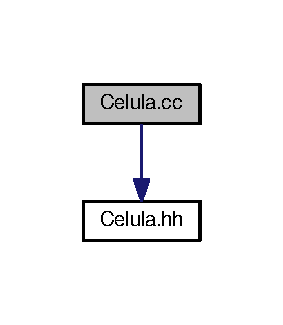
\includegraphics[width=136pt]{_celula_8cc__incl}
\end{center}
\end{figure}


\subsection{Descripción detallada}
Código de la clase \hyperlink{class_celula}{Celula}. 


\hypertarget{_celula_8hh}{}\section{Referencia del Archivo Celula.\+hh}
\label{_celula_8hh}\index{Celula.\+hh@{Celula.\+hh}}


Especificación de la clase \hyperlink{class_celula}{Celula}.  


\subsection*{Clases}
\begin{DoxyCompactItemize}
\item 
class \hyperlink{class_celula}{Celula}
\begin{DoxyCompactList}\small\item\em Representa el conjunto de características y operaciones de las células. \end{DoxyCompactList}\end{DoxyCompactItemize}


\subsection{Descripción detallada}
Especificación de la clase \hyperlink{class_celula}{Celula}. 


\hypertarget{_organismo_8cc}{}\section{Referencia del Archivo Organismo.\+cc}
\label{_organismo_8cc}\index{Organismo.\+cc@{Organismo.\+cc}}


Código de la clase \hyperlink{class_organismo}{Organismo}.  


Dependencia gráfica adjunta para Organismo.\+cc\+:\nopagebreak
\begin{figure}[H]
\begin{center}
\leavevmode
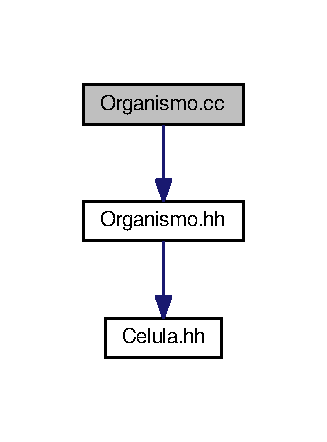
\includegraphics[width=157pt]{_organismo_8cc__incl}
\end{center}
\end{figure}


\subsection{Descripción detallada}
Código de la clase \hyperlink{class_organismo}{Organismo}. 


\hypertarget{_organismo_8hh}{}\section{Referencia del Archivo Organismo.\+hh}
\label{_organismo_8hh}\index{Organismo.\+hh@{Organismo.\+hh}}


Especificación de la clase \hyperlink{class_organismo}{Organismo}.  


Dependencia gráfica adjunta para Organismo.\+hh\+:\nopagebreak
\begin{figure}[H]
\begin{center}
\leavevmode
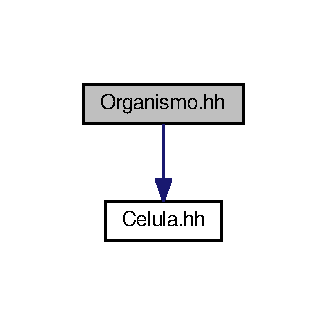
\includegraphics[width=157pt]{_organismo_8hh__incl}
\end{center}
\end{figure}
\subsection*{Clases}
\begin{DoxyCompactItemize}
\item 
class \hyperlink{class_organismo}{Organismo}
\begin{DoxyCompactList}\small\item\em Representa la información y las operaciones asociadas a un organismo. \end{DoxyCompactList}\end{DoxyCompactItemize}


\subsection{Descripción detallada}
Especificación de la clase \hyperlink{class_organismo}{Organismo}. 


\hypertarget{pro2_8cc}{}\section{Referencia del Archivo pro2.\+cc}
\label{pro2_8cc}\index{pro2.\+cc@{pro2.\+cc}}


Programa principal.  


Dependencia gráfica adjunta para pro2.\+cc\+:\nopagebreak
\begin{figure}[H]
\begin{center}
\leavevmode
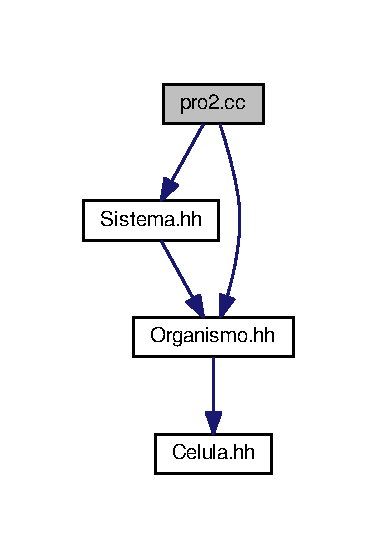
\includegraphics[width=181pt]{pro2_8cc__incl}
\end{center}
\end{figure}
\subsection*{Funciones}
\begin{DoxyCompactItemize}
\item 
int \hyperlink{pro2_8cc_ae66f6b31b5ad750f1fe042a706a4e3d4}{main} ()
\end{DoxyCompactItemize}


\subsection{Descripción detallada}
Programa principal. 

Estamos suponiendo que los datos leídos siempre son correctos, ya que no incluímos comprobaciones al respecto. Por último, puesto que los datos de los organismos y células son naturales (identificadores, ...) usaremos números negativos para las opciones. 

\subsection{Documentación de las funciones}
\index{pro2.\+cc@{pro2.\+cc}!main@{main}}
\index{main@{main}!pro2.\+cc@{pro2.\+cc}}
\subsubsection[{\texorpdfstring{main()}{main()}}]{\setlength{\rightskip}{0pt plus 5cm}int main (
\begin{DoxyParamCaption}
{}
\end{DoxyParamCaption}
)}\hypertarget{pro2_8cc_ae66f6b31b5ad750f1fe042a706a4e3d4}{}\label{pro2_8cc_ae66f6b31b5ad750f1fe042a706a4e3d4}


Definición en la línea 45 del archivo pro2.\+cc.


\begin{DoxyCode}
46 \{
47   \textcolor{keywordtype}{int} N; \textcolor{comment}{//  Número de parámetros de las células}
48   cin >> N; 
49   \hyperlink{class_sistema}{Sistema} S;
50   S.\hyperlink{class_sistema_ae670549104642dd4664ac8f794b4b1e9}{leer}(N);
51   \textcolor{keywordtype}{int} op; \textcolor{comment}{// Código de operación}
52   cin >> op;
53   \textcolor{keywordflow}{while} (op != -3) \{
54     \textcolor{keywordflow}{if} (op == -1 ) \{
55       \hyperlink{class_organismo}{Organismo} O;
56       O.\hyperlink{class_organismo_a189d611401e25f603103c420d0b62e23}{leer}(N);
57       \textcolor{keywordtype}{bool} sobrevive;
58       S.\hyperlink{class_sistema_a6522b718fc0701d38c2e2d2c2d2e88a6}{anadir\_organismo}(O, sobrevive);
59       cout << \textcolor{stringliteral}{"Entrada del nuevo organismo"} << endl;
60       cout << O.\hyperlink{class_organismo_aadcc0750f9405e7334ac6a69e4ebb1b8}{num\_victimas}() << \textcolor{stringliteral}{" "} << sobrevive << endl;  
61     \} 
62     \textcolor{keywordflow}{else} \textcolor{keywordflow}{if} (op == -2) \{
63       \textcolor{keywordtype}{bool} tipo = readbool();     
64       \textcolor{keywordtype}{bool} estr = readbool();
65       \textcolor{keywordflow}{if} (tipo)\{
66   \textcolor{keywordflow}{if} (estr) cout << \textcolor{stringliteral}{"Defensivos del sistema con estructura"} << endl;  
67   \textcolor{keywordflow}{else} cout << \textcolor{stringliteral}{"Defensivos del sistema sin estructura"} << endl;
68       \}
69       \textcolor{keywordflow}{else} \{
70   \textcolor{keywordflow}{if} (estr) cout << \textcolor{stringliteral}{"Malignos del sistema con estructura"} << endl;
71   \textcolor{keywordflow}{else} cout << \textcolor{stringliteral}{"Malignos del sistema sin estructura"} << endl;
72       \}
73       S.\hyperlink{class_sistema_a3f2a05a17345ee3be8331950fb2eedc0}{escribir}(tipo, estr);
74     \}
75     cin >> op;
76   \}
77 \}
\end{DoxyCode}

\hypertarget{_sistema_8cc}{}\section{Referencia del Archivo Sistema.\+cc}
\label{_sistema_8cc}\index{Sistema.\+cc@{Sistema.\+cc}}


Código de la clase \hyperlink{class_sistema}{Sistema}.  


Dependencia gráfica adjunta para Sistema.\+cc\+:\nopagebreak
\begin{figure}[H]
\begin{center}
\leavevmode
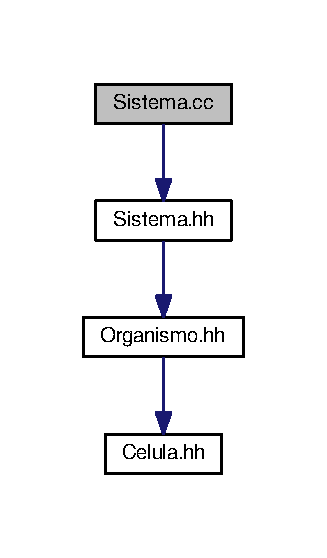
\includegraphics[width=157pt]{_sistema_8cc__incl}
\end{center}
\end{figure}


\subsection{Descripción detallada}
Código de la clase \hyperlink{class_sistema}{Sistema}. 


\hypertarget{_sistema_8hh}{}\section{Referencia del Archivo Sistema.\+hh}
\label{_sistema_8hh}\index{Sistema.\+hh@{Sistema.\+hh}}


Especificación de la clase \hyperlink{class_sistema}{Sistema}.  


Dependencia gráfica adjunta para Sistema.\+hh\+:\nopagebreak
\begin{figure}[H]
\begin{center}
\leavevmode
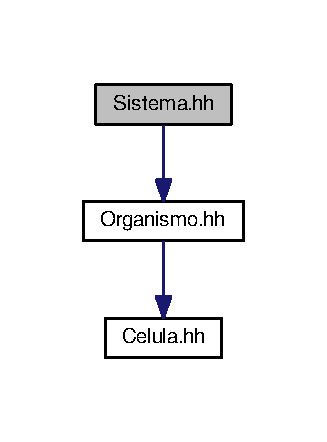
\includegraphics[width=157pt]{_sistema_8hh__incl}
\end{center}
\end{figure}
\subsection*{Clases}
\begin{DoxyCompactItemize}
\item 
class \hyperlink{class_sistema}{Sistema}
\begin{DoxyCompactList}\small\item\em Representa el sistema donde se desarrollan los experimentos. \end{DoxyCompactList}\end{DoxyCompactItemize}


\subsection{Descripción detallada}
Especificación de la clase \hyperlink{class_sistema}{Sistema}. 


%--- End generated contents ---

% Index
\backmatter
\newpage
\phantomsection
\clearemptydoublepage
\addcontentsline{toc}{chapter}{Índice}
\printindex

\end{document}
